\documentclass{report}
\usepackage[utf8]{inputenc}

% **********************************************************
% Document Settings                                        *
% **********************************************************
\usepackage{geometry}
\geometry{a4paper, margin=0.6in}

\usepackage{graphicx}
\graphicspath{{../outputs/}}

\usepackage{minted}
% \usemintedstyle{emacs}

\usepackage{fancyhdr}
\pagestyle{fancy}
\fancyhf{}
\lhead{Java Programming}
\rhead{Suman Mondal}
% \lfoot{\href{https://github.com/thatsuman/ccpcst-assignment.git}{View on Github}}
\lfoot{\href{https://github.com/thatsuman}{DCCPCSTS6 - 10005537}}
\rfoot{Page \thepage}

\usepackage{hyperref}
\hypersetup{
colorlinks=true,
linkcolor=blue,
filecolor=magenta,
urlcolor=blue,
}
\urlstyle{same}

\usepackage{fontspec}
% \setromanfont{Source Sans Pro}
% \setmonofont{Cascadia Code PL}


% macros start here
\newcommand{\problem}[3]{
  \section{#3}
    \underline{{\LARGE Source Code :}}
    \inputminted[breaklines,fontsize=\Large]{java}{#1.java}
    \bigbreak
    \noindent
    \underline{{\LARGE Program Output :}}
    \bigbreak
    \noindent
    \includegraphics[width=100mm,scale=0.5]{#2}
% \newpage
}
\newcommand{\subproblem}[3]{
  \subsection{#3}
    \underline{\emph{\Large Source Code :}}
    \inputminted[breaklines]{java}{#1.java}
    \bigbreak
    \noindent
    \underline{\emph{\Large Program Output :}}
    \bigbreak
    \noindent
    \includegraphics[width=110mm,scale=0.5]{#2}
% \newpage
}
% macros end here

% **********************************************************

\begin{document}
\begin{titlepage}
  \begin{center}
    \vspace*{2cm}
    
\includegraphics[width=0.3\textwidth]{logo}\\
    \vspace{0.5cm}
    {\huge \textbf{CENTRAL CALCUTTA POLYTECHNIC}}\\
    \vspace{0.4cm}
    21, Convent Road, Philips, Sealdah, Kolkata, West Bengal 700014\\
    \vspace{0.8cm}
    {\Large \textsc{dept. : computer science and technology}}
  \end{center}
  \vspace{1.2cm}
  \textsc{
    \huge
    \begin{itemize}
      \item name : suman mondal
      \item roll : dccpcsts5
      \item number : 10005537
      \item reg number : d192005242
      \item subject : java programming
      \item session : 2021 - 2022
      \item email : suman.mondal@outlook.in
    \end{itemize}
  }

\end{titlepage}

\pagenumbering{roman}
\newpage
\large{\tableofcontents}
% \tableofcontents
\clearpage
\pagenumbering{arabic}

\chapter{AWT}
\problem{../codes/awt/Q01}{awt/Q01}{Frame with Title and Label}
\problem{../codes/awt/Q02}{awt/Q02}{Adding Button and Flow Layout}
\problem{../codes/awt/Q03}{awt/Q03}{Adding Grid Layout}
\problem{../codes/awt/Q04}{awt/Q04}{Create Login Form}
\problem{../codes/awt/Q05}{awt/Q05}{Adding Border Layout}
\problem{../codes/awt/Q06}{awt/Q06}{Calculator Using Panel}
\problem{../codes/awt/Q07}{awt/Q07}{Adding Checkbox}
\problem{../codes/awt/Q08}{awt/Q08}{Copy a Textfield Content to Another Textfield Using Event Handling}
\problem{../codes/awt/Q09}{awt/Q09}{Textfield Content Always in Upper Case}
\problem{../codes/awt/Demoevent}{awt/Q10.1}{User Details Entry using AWT Textfield, Checkbox Group, Choice Object and Event Handling}
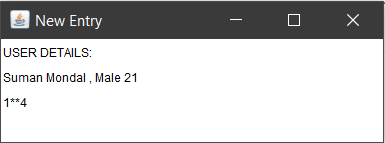
\includegraphics[width=100mm,scale=0.5]{awt/Q10.2.PNG}

\chapter{Socket Programming}
\section{TCP Socket Program}
\subproblem{../codes/socket/Q01ServerSide}{socket/Q01Server}{Server Side}
\subproblem{../codes/socket/Q01ClientSide}{socket/Q01Client}{Client Side}

\section{TCP Socket Program for Multiple Client using Threads}
\subproblem{../codes/socket/Q02ServerSide}{socket/Q02Server}{Server Side}
\subproblem{../codes/socket/Q02ClientSide}{socket/Q02Client}{Client Side}

\section{UDP Socket Program}
\subproblem{../codes/socket/Q03ServerSide}{socket/Q03Server}{Server Side}
\subproblem{../codes/socket/Q03ClientSide}{socket/Q03Client}{Client Side}

\chapter{Swing}
\problem{../codes/swing/Q01}{swing/Q01}{JPasswordField}
\problem{../codes/swing/Q02}{swing/Q02}{JTable}
\problem{../codes/swing/Q03}{swing/Q03}{JPasswordField}

\end{document}

